\documentclass[8pt]{article} 

% Formatting:
% -----------------------------------------------------------------------------------------------
\setlength{\oddsidemargin}{0cm} 
\setlength{\topmargin}{0cm}
\setlength{\textheight}{21cm}
\setlength{\textwidth}{16.0cm}
\setlength{\columnwidth}{16.0cm} 

% Packages:
% -----------------------------------------------------------------------------------------------
\usepackage[intlimits]{amsmath}
\usepackage{amssymb}
\usepackage{amsfonts}
\usepackage{amsthm}
\usepackage{latexsym}
\usepackage{epsfig}
\usepackage{color}
\usepackage{float}
\usepackage{graphicx}
\usepackage{fancyhdr}
\usepackage{lipsum} 
\usepackage{listings}

\usepackage{array}
\usepackage{booktabs}
\usepackage{courier}
\usepackage{mdframed}
\usepackage{pgfgantt}
\usepackage{rotating}
\usepackage{titling}
\usepackage{url}
\usepackage{verbatim}
\usepackage[margin=50pt,font=small,labelfont=bf]{caption}

\usepackage{pdfpages}
\graphicspath{figures}
%\usepackage{relsize}
%\usepackage{tikz}

%listings stuff
% -----------------------------------------------------------------------------------------------
\lstset{basicstyle=\footnotesize\ttfamily,breaklines=true}
%\lstset{framextopmargin=50pt,frame=bottomline}
\lstset{framextopmargin=50pt}


% Table Shit from Bidski
% ------

\newcolumntype{L}[1]{>{\raggedright\let\newline\\\arraybackslash\hspace{0pt}}m{#1\textwidth}}
\newcolumntype{C}[1]{>{\centering\let\newline\\\arraybackslash\hspace{0pt}}m{#1\textwidth}}
\newcolumntype{R}[1]{>{\raggedleft\let\newline\\\arraybackslash\hspace{0pt}}m{#1\textwidth}}

% Theorem environments:
% -----------------------------------------------------------------------------------------------
\newtheorem{thm}{Theorem}
\newtheorem{prp}{Proposition}
\newtheorem{cor}{Corollary}
\newtheorem{lem}{Lemma}
\newtheorem{df}{Definition}
\newtheorem{alg}{Algorithm}
\newtheorem{con}{Conjecture}

\graphicspath {figs/} 

\pdfpagewidth 8.5in
\pdfpageheight 11in

\pagestyle{fancy}

\lhead{COMP3851A - CompSci Work Integrated Learning Part A}
\chead{}
\rhead{Project Plan Report}
%\rfoot{Right bottom}
\cfoot{\thepage}
%\lfoot{Left bottom}

% Commands
% -----------------------------------------------------------------------------------------------
\newcommand{\inftyint}{\int_{-\infty}^{+\infty}}
\newcommand{\unit}[1]{\ensuremath{\, \mathrm{#1}}}

\newcommand{\executeiffilenewer}[3]{%
\ifnum\pdfstrcmp{\pdffilemoddate{#1}}%
{\pdffilemoddate{#2}}>0%
{\immediate\write18{#3}}\fi%
}
\newcommand{\includesvg}[1]{%
\executeiffilenewer{#1.svg}{#1.pdf}%
{inkscape -z -D --file=#1.svg %
--export-pdf=#1.pdf --export-latex}%
\input{#1.pdf_tex}%
}

% -----------------------------------------------------------------------------------------------



\begin{document}
\numberwithin{equation}{section}

%
% ---- TITLE ------------------------------------------------------------------------------------
% -----------------------------------------------------------------------------------------------
%

%      %%%
%     %%%%
%    %%%%%
%   %%%%%%
%      %%%
%      %%%
%      %%%
%      %%%
%      %%%
%      %%%
%   %%%%%%%%%
%   %%%%%%%%%
%
%
% ---- INTRODUCTION -----------------------------------------------------------------------------
% -----------------------------------------------------------------------------------------------
%

\title{
	
\includegraphics[scale=0.5]{UON_Logo}
	\vspace{60pt}
	\\COMP3851A - CompSci Work Integrated Learning Part A
	\\ \textbf {Remote Control Car learns to drive using Machine Learning}
	\\ \textbf {Project Plan }  
}
\author{
	Jordan Haigh (c3256730), Evan Gresham (c3196094), Mathew Rixon (c3274723) \\
	The University of Newcastle, Australia\\
}
%\date{Last Revision: \today}
% -----------------------------------------------------------------------------------------------


\maketitle

\newpage

%      %%%%%
%    %%%%%%%%%
%   %%%     %%%
%           %%%
%           %%%
%      %%%%%%%
%    %%%%%%%
%   %%%
%   %%%
%   %%%
%   %%%%%%%%%%%
%   %%%%%%%%%%%
%
%
% -----------------------------------------------------------------------------------------------
%

\section{Summary}
Self driving cars are no longer a thing of the future, we have them here and now, however the Artificial intelligence in these vehicles requires thousands of hours of training data and millions of lines of code, where the developers directly show the the AI how to act. Our team believes this to be excessively onerous. During this project our team intends to have a car learn to drive all by itself, through the process of trial and error. The only difference between us and Tesla is that the cars we will be working on are slightly smaller.  
\\\\
The team will attach a Raspberry Pi to a remote control car and have it learn to drive using current methods in reinforcement learning. The team will also deliver a virtual simulation of the car which will allow us to easily implement and compare multiple popular algorithms in machine learning.





%\begin{mdframed}
%\noindent \textbf{Notes:}
%	
%\textit{Remember}, Fusce ante mauris, semper at ligula a, aliquam placerat justo. Proin eu lacinia orci. Nunc fermentum, enim ac tempus mollis, justo turpis dapibus odio, nec ultricies elit lorem nec ligula. Vivamus at tellus at ligula sodales congue eu vel orci. Vestibulum euismod dapibus mauris vehicula interdum. Curabitur id vehicula tortor, vel pretium erat. Proin congue, purus placerat sagittis ultricies, nisi erat imperdiet eros, in lacinia lorem erat at lectus. Interdum et malesuada fames ac ante ipsum primis in faucibus.
%
%\end{mdframed} 

\section {Background}
\subsection{Robotics}
Currently one of the main focuses of AI in the industry is receiving information from the environment and processing it. Tools such as image classifiers and speech translators are well used features in modern society. The team is interested in the inverse, applying artificial intelligence in a way that can interact back with the environment. This includes self-driving cars and humanoid robots. Self-driving cars already exist and have progressed rapidly in the last few years, and robots that mimic human motion and behaviour are also making huge strides forward.

\subsection{Artificial Intelligence and Reinforcement Learning}
Our team has a keen interest in artificial intelligence and its’ applications in robotics. During our time at university, each team member has completed a Machine Intelligence course, which provided insight into the different types of Artificial Intelligence and what they can achieve.
\\\\
During this project the team will implement and compare many modern methods in the field of Artificial intelligence. Traditionally supervised learning methods have provided superior results, however more recently, reinforcement learning algorithms have surfaced and have started to become more widely used. The reinforcement learning method that our team will explore is known as Q-learning and Deep Q-learning. Q-learning is a model-free reinforcement learning algorithm which can learn an optimal policy for any Markov Decision Problem (discrete-time stochastic control process)\cite{MarkovDecisionProcess} with a finite input space. The algorithm creates a Q-table which stores the values of each state-action pair. This table is updated as the agent explores the environment through a trial and error approach. As previously stated, this algorithm only works on a finite input space, this is why Deep Q Learning was developed. Deep Q-Learning uses a Neural Network in place of the Q-table which acts as a function approximator mapping state-action pairs to their value. 
\\\\
Deep Q-Learning (DQL) was popularised in 2015 when a paper was published \cite{DeepQLearningReleasePaper} demonstrating DQL achieving close to human level of play on the entire suite of ATARI games. Since then, many improvements to the DQL algorithm have been developed, including double DQL,  prioritised replay buffer and dueling DQL.
\\\\
Artificial Intelligence is widely used throughout modern society, from object detection to big data analysis.

\newpage


%
% -----------------------------------------------------------------------------------------------
%

%      %%%%%
%    %%%%%%%%%
%   %%%     %%%
%           %%%
%           %%%
%      %%%%%%%
%      %%%%%%%
%           %%%
%           %%%
%   %%%     %%%
%    %%%%%%%%%
%      %%%%%
%
%
% -----------------------------------------------------------------------------------------------
%

\subsection{Self-Driving Cars}
Self-driving cars are one of the most talked about things in the world of modern AI. The technology is to the point where it really is self-driving. The first applications of self-driving features were however far more minor.
\\\\
The first feature considered to be self-driving was the cruise control feature, it was invented in 1948 \cite{CruiseControl} and the main purpose of it was to maintain the speed of the car without the need for input from the driver. It was simple in that it would only do the speed of the car when the feature was activated. After that, it progressed to adaptive cruise control, where a car is outfitted with sensors and is able to speed up and slow down with the flow of traffic, again without input from the driver. Slowly many separate features such as lane assist, park assist, proximity alerts etc all made their way into cars, and eventually all integrated together along with new AI algorithms. With modern self driving cars, there are many advanced sensors all around the car to take in its environment, and powerful computers making decisions on what to do next. 
\\\\
The modern age of self driving cars started around 2009 with the \emph{Google Waymo Project} \cite{WaymoProject}, and was limited to uninterrupted driving on straight highways for only about 10-100 miles. Self-driving really gained public attention in 2014 with Elon Musk’s Tesla cars being kitted with their newest Autopilot system \cite{TelstraAutopilot}. Since then many companies have join in the race to make the first fully automated car. Unfortunately much of this progress is limited by legal barriers. Many countries still forbid self-driving completely, or severely limit it, despite current autonomous technology being statistically safer than the average human driver.


\subsection{Problems in the Area}
A common problem when working with Machine Intelligence is determining whether these algorithms are able to generalise beyond its training scenarios. Many argue that there are far too many variational occurrences in reality, making it impossible to train an algorithm and flawlessly cope with new problems. The team will be exploring generalisation in this project in order to solve any overfitting issues that may arise. 

\newpage

%          %%%
%         %%%
%        %%%
%       %%%
%      %%%
%     %%% %%%
%    %%%  %%%
%   %%%%%%%%%%%
%   %%%%%%%%%%%
%         %%%   
%         %%%   
%         %%%    
%
%
% -----------------------------------------------------------------------------------------------
%


\section{Aims / Expected Outcomes}

\subsection{Aims}
\begin{itemize}
	\item Create a simulated environment in software to closely resemble the real world functionality of the selected vehicle.
	\begin{itemize}
		\item Accurately model the vehicle and its behaviour.
		\item Build a virtual track to test the vehicle in.
		\item Simulate required physics to allow for an accurate simulation of the motion of the vehicle.
	\end{itemize}

	\item Implement Machine Learning and Artificial Intelligence algorithms in the simulated environment.
	\begin{itemize}
		\item Condition-Based Algorithm
		\item Evolutionary Algorithm
		\item Q-learning
		\item Deep Q-learning
		\item PPO
	\end{itemize}

	\item Compare and contrast current algorithms in Machine Learning and Artificial Intelligence based on their performance and efficiency.

	\item Select the most appropriate algorithm to implement in the real world RC Car example

	\item Interface a Raspberry Pi with the selected remote control vehicle to allow intelligent control of the vehicle.

	\item Add required sensors to the Raspberry Pi. e.g. ultrasonic distance sensor, accelerometer.

	\item Implement the chosen Machine Learning algorithm on the Raspberry Pi controlling the vehicle.
	
	\item Construct a physical track from materials which is easily modifiable, cheap and sturdy.  
	
	\item Have a remote control car drive autonomously around a physical track utilising learned behavior.
\end{itemize}

\subsection{Expected Outcomes}
The team will deliver a program which accurately simulates the physics and movement of the real world car. This program will be developed using a 3D virtual environment creator called Unity \cite{Unity3D}. This program has the functionality available to create a variety of simulations, model the car in three dimensions and create tracks to test/ train the car on. 
\\\\
By generating a large number of training tracks, the chances of the AIs overtraining on a specific track will be significantly reduced. This will encourage the AI algorithms to learn generalised behaviour patterns, with the ability to cope with previously unseen tracks.
\\\\
Another functionality of the simulation is the ability to test a series of Artificial Intelligence algorithms in our test environment. This will allow the team to observe and select the most successful algorithm and apply to the real life car. The observation process will also serve as a study comparing the positives and negatives of each algorithm. 
\newpage



%   %%%%%%%%%%%
%   %%%%%%%%%%%
%   %%% 
%   %%%
%   %% %%%%%
%   %%%%%%%%%%
%           %%%
%           %%%
%           %%%
%   %%%     %%%
%    %%%%%%%%%
%      %%%%%
%
%
% -----------------------------------------------------------------------------------------------
%
The simulation program must additionally imitate the sensors which will be attached to the RC car. This ensures that the algorithms will perform similarly in the simulation and in reality, since the sensory inputs will be identical.
\\\\
The first algorithm to test and apply to the cars is a simple conditional based algorithm. This will check the distance to the left and right and if either is too close it will turn in the opposite direction. This is the most basic algorithm to be implemented, it will work as a test ensuring the simulation works properly and to establish a base case for comparing the other algorithms to.
\\\\
The second algorithm to be tested is evolving an Artificial Neural Network \emph{(ANN)} to drive through the courses using the evolutionary algorithm. This algorithm will be more difficult to implement on the real car because it requires a large population to be functional (the team has only one prototype vehicle). 
\\\\
It is hypothetically possible to test every car in a generation one at a time, however this would become a time-consuming process - the car would need to be reset after each populant is tested, inferring this algorithm would require a large amount of human intervention. This must be considered before selecting this algorithm.
\\\\
The third algorithm to be implemented is tabular Q-Learning. This algorithm cannot work on a near infinite input space (which the distance sensors will provide), so the input distances will need to be divided into a small number of brackets in order to be able to tabulate the state space. This algorithm can be tweaked to work with the near infinite input space if we introduce Neural Networks. This tweaked algorithm is called deep Q-Learning.
\\\\
If we have enough time, another algorithm may be considered. Proximal Policy Optimisation (PPO) is currently a state-of-the-art reinforcement learning algorithm. However, no team member has any experience with this algorithm, implementing this algorithm will be challenging. If the team is not able to write the PPO algorithm, the usage of libraries will be considered.
\\\\
The second part of this project is to implement the chosen Machine Learning algorithm on a remote control car. The team will deliver an RC car with an integrated Raspberry Pi. The vehicle will have multiple distance sensors mounted such that the algorithms can receive sensory information about its environment and act intelligently. The chosen Machine Learning algorithm will be implemented on the Raspberry Pi for the car to drive autonomously.
\\\\
A physical track will be constructed with a material that is cheap and modifiable. This track is necessary in order to train the AI in the real word. The chosen material will need to be sturdy enough to withstand the car colliding with it aperiodically. As with generating multiple tracks in the software simulation, the team will train the car on multiple tracks.
\\\\
Finally, the team will test the algorithm and deliver the RC car with a learned policy and documentation of the learning process through an edited video, compiling footage of the Artificial Intelligence algorithm learning an optimal policy.

\subsection{Team Experience / Skills}
There are two main aspects of this project: software/AI and hardware. Our team consists of members with experience in both of these areas. Apart from the PPO algorithm mentioned previously, our team has experience in implementing all other Machine Learning algorithms. 

\newpage



%      %%%%%
%    %%%%%%%%%
%   %%%     %%%
%   %%%
%   %% %%%%%
%   %%%%%%%%%%
%   %%%     %%%
%   %%%     %%%
%   %%%     %%%
%   %%%     %%%
%    %%%%%%%%%
%      %%%%%
%
%
% -----------------------------------------------------------------------------------------------
%

The simulation will be created using the Unity3D development engine, all team members have some experience with this engine although further learning will be required to create a program of this complexity. This isn't a major concern as there is a plethora of resources online for learning this engine, as well as allocating time in the timeline for members to complete this training.
\\\\
The hardware component of this project is mostly alien to our team. Our team has a member who has experience with Raspberry Pis and using electronics to control hardware components. This member will handle most of the integration of the Raspberry Pi with the RC car while the other two members will handle building the software simulation.
\\\\
Whilst some learning is required by its members, the team is confident in the expertise required to achieve these aims and deliver the expected outcomes within the time allocated.


\section{Approach}
\subsection{Computers and Electronics Hardware}
The computer we will be attaching to the car is the Raspberry Pi 3 Model B+. This computer is very powerful for such a small device, with the capability to run full Operating Systems. This will close the gap between writing high level code (selecting from a variety of programming languages and AI libraries) and connecting to GPIO pins (handling sensors and interfacing with the remote control car).
\\\\
There may be some parts of the interface between the Raspberry Pi and the car's electronics that the Raspberry Pi may not be able to perform correctly or efficiently enough. If these cases should occur, the team will improve the performance by coupling it with an Arduino UNO. This device is known for it’s real time nature, making it ideal for many types of robotics.


\begin{figure}[h]
	\centering
	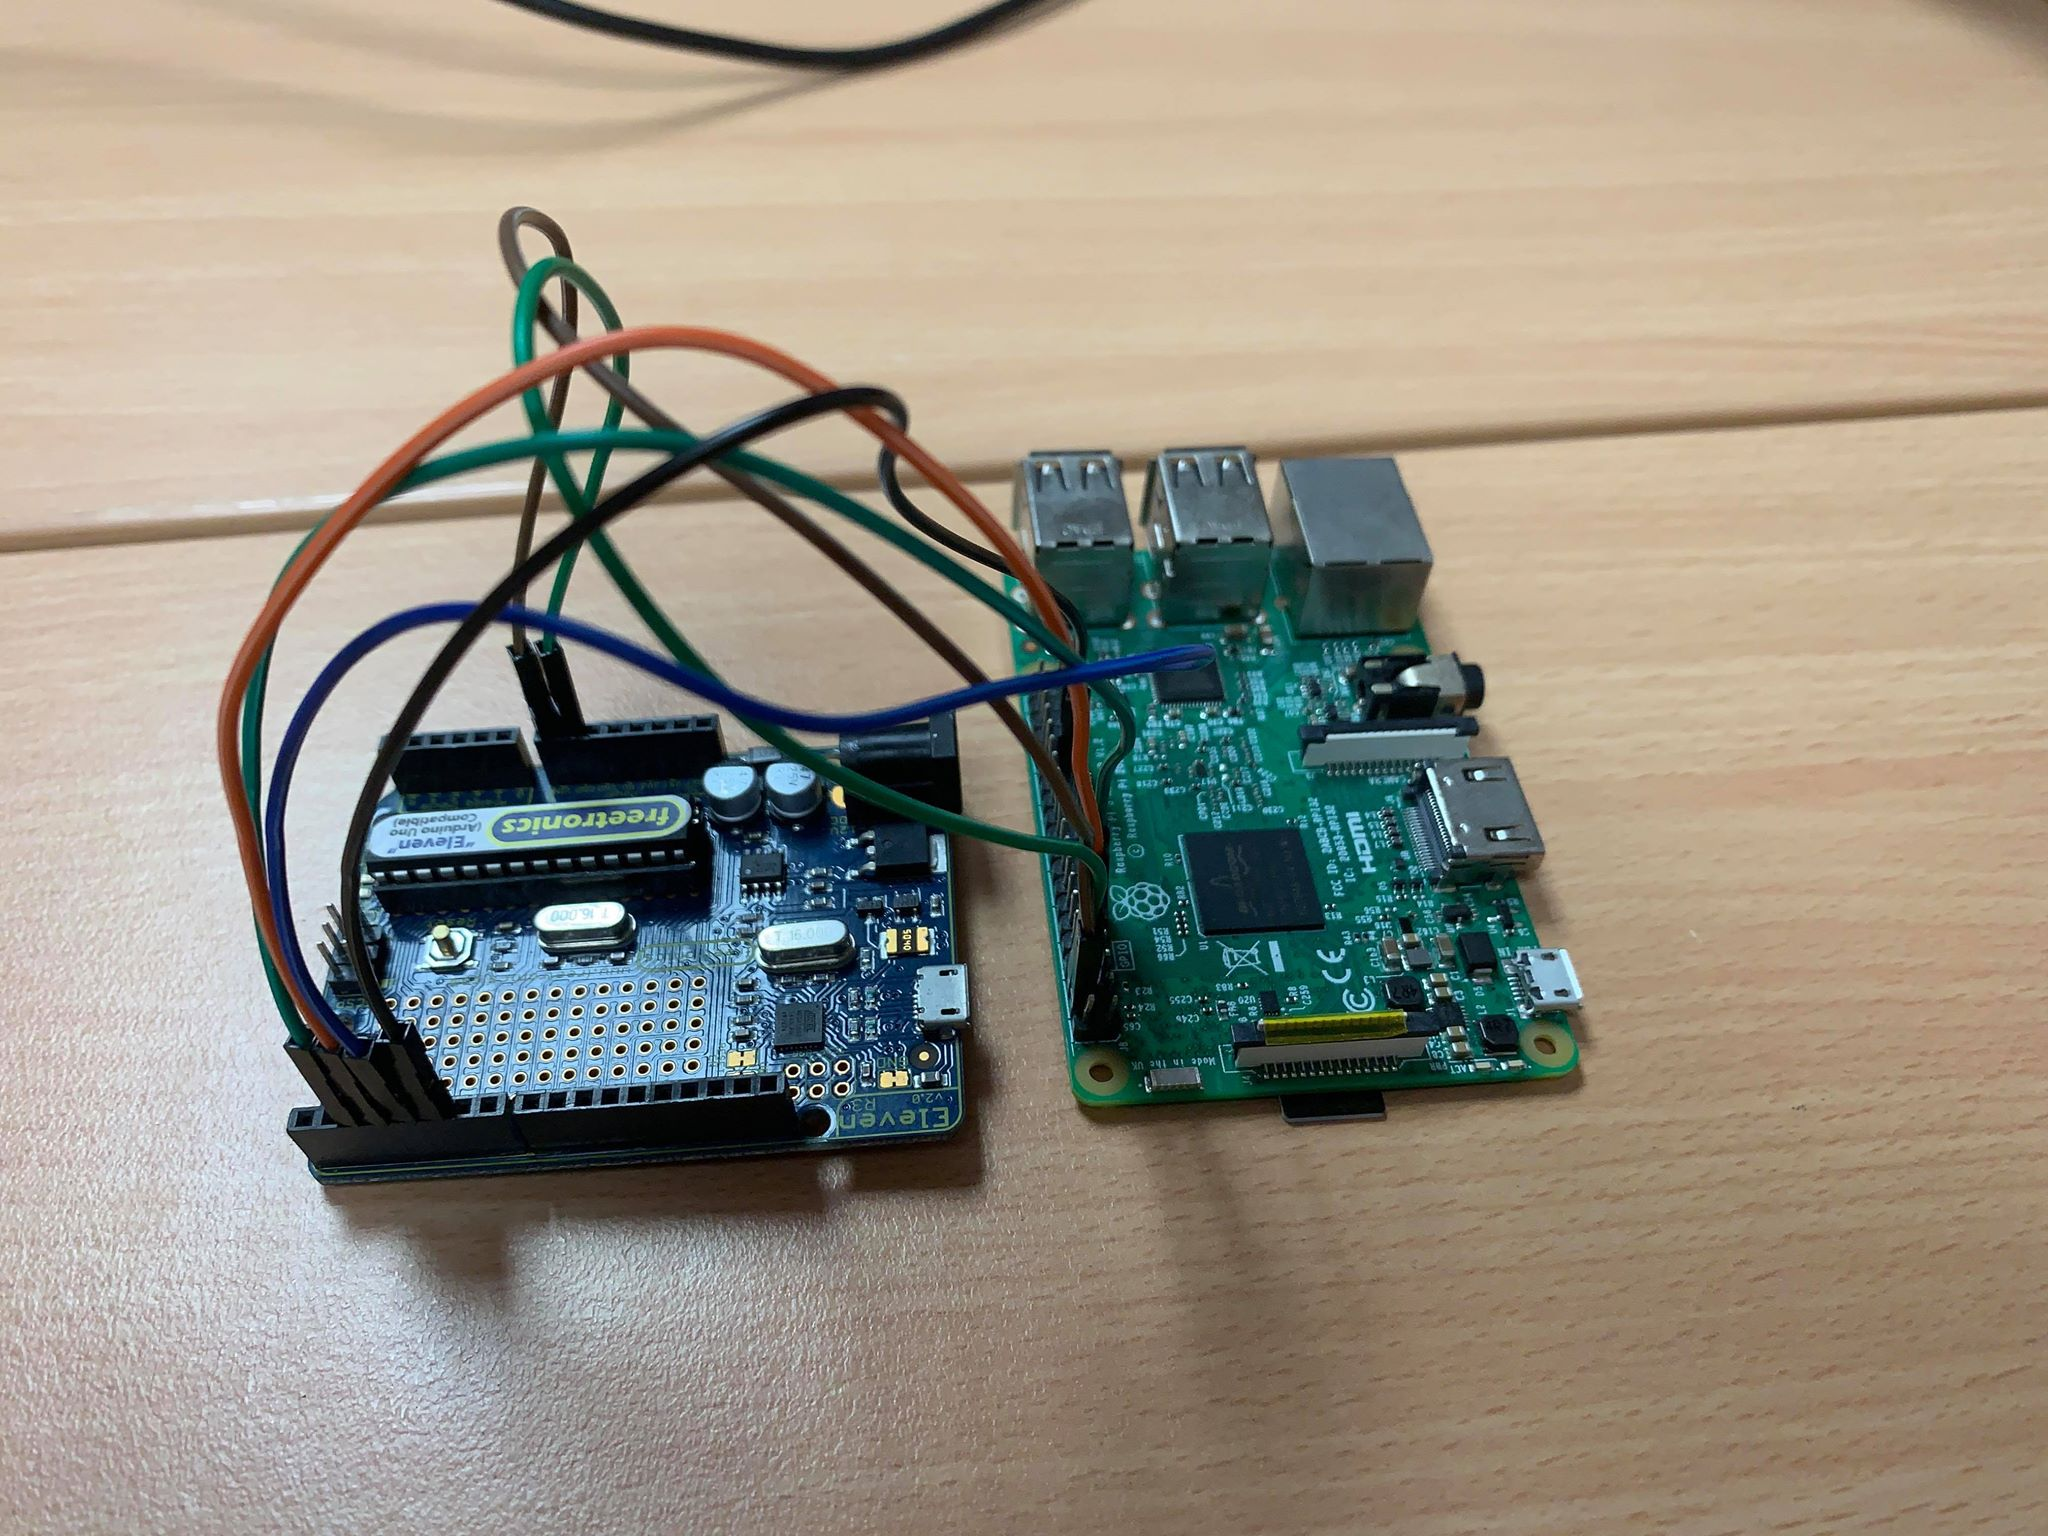
\includegraphics[height=7cm, width=7cm]{figures/TwoBoards.jpg}
	\caption{Two Electronic Boards - \emph{Left:}Arduino UNO, \emph{Right:} Raspberry Pi}
	\label{fig:AruinoUNORaspberryPi} 	
\end{figure}

%   %%%%%%%%%%%
%   %%%%%%%%%%%
%           %%%
%           %%%
%          %%%
%         %%%
%        %%%
%       %%%
%       %%%
%       %%% 
%       %%%
%       %%%
%
%
% -----------------------------------------------------------------------------------------------
%
The Raspberry Pi will interface with the RC car directly by connecting the GPIO pins to the controller board inside the car. This method will minimise any latency issues, which is critical for reaction time and obstacle avoidance for the Artificial Intelligence.
\\\\
The sensors the team will be using are the HC-SR04 Ultrasonic Distance sensors. These sensors are accurate to millimeters and have very negligible response latency. This makes it an ideal choice as the distance between the car and objects will be used as environmental input data for the AI to continue training and improving it’s model.
\\
\begin{figure}[h]
	\centering
	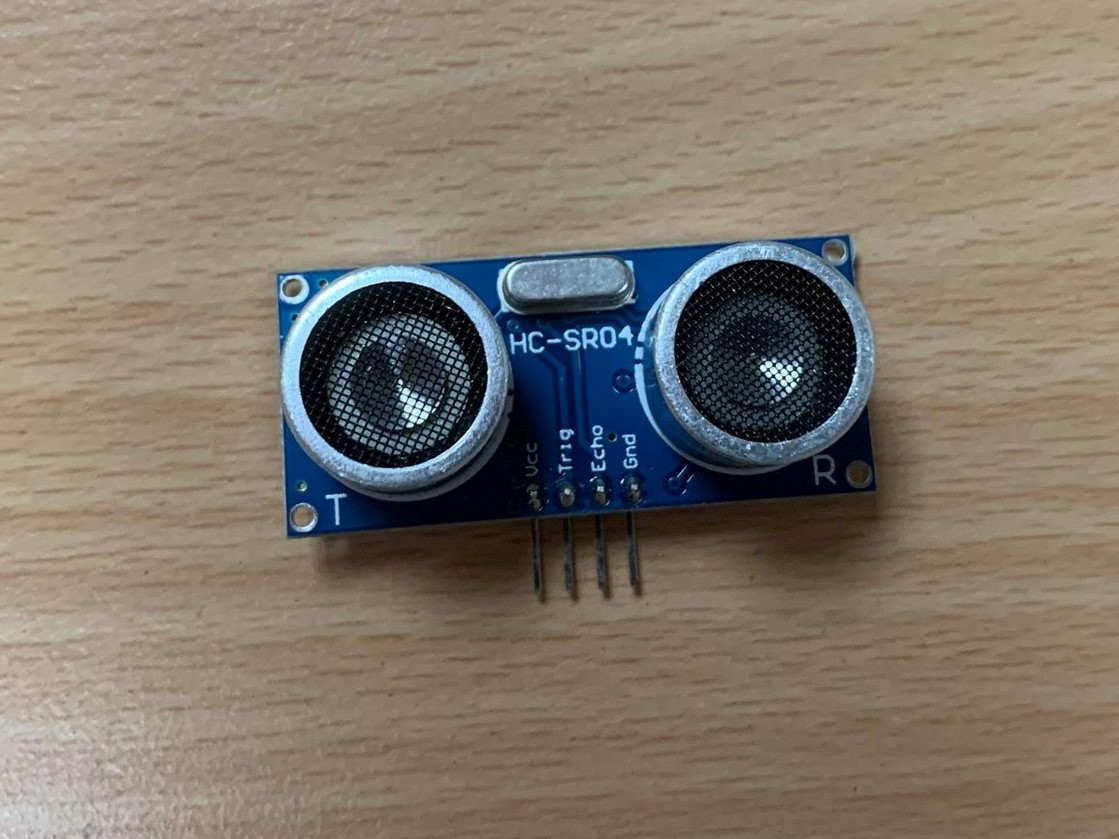
\includegraphics[height=5cm, width=5cm]{figures/DistanceSensor2.jpg}
	\caption{HC-SR04 Ultrasonic Distance Sensor}
	\label{fig:DistanceSensor} 	
\end{figure}


\subsection{Robotics}
For this project, the team will be modifying an existing Remote Control (RC) Car so that it can be controlled from an onboard computer mounted to the car.
There was the option to build the locomotion robot ourselves, though with careful thought and discussion, it was decided that purchasing a retail Remote Control Car was far more beneficial. 
The considerations that led us to the conclusion of purchasing a retail version included:

\begin{itemize}
	\item \textbf{Simplicity} - Given that our team has limited to no previous experience with robotics, it would be unrealistic for us to develop an effective robot within the time frame needed.
	\item \textbf{Consistency} - If an electronic part failed and needed to be replaced, the team has no guarantee (given our skill sets) that a part could be repaired, or recreate an section of the vehicle corresponding to the original blueprint. Certain alterations could affect the weight or mobility of the vehicle and not work with a pre-existing AI model. A drastic change could force our team to retrain the AI and vehicle with new parameters. A retail remote control car does not have this issue; the team can buy another off-the-shelf vehicle and be assured it will function similarly to the previous car.
	\item \textbf{Cost and Time} - Building something ourselves (given our experience level) would lead to a higher budget consideration and less time resources. Or on the other hand, spending more time to design a cheaper vehicle, which is still not efficient with time. Existing retail RC cars are relatively cheap and good quality for the price.
\end{itemize}
\begin{figure}[h]
	\centering
	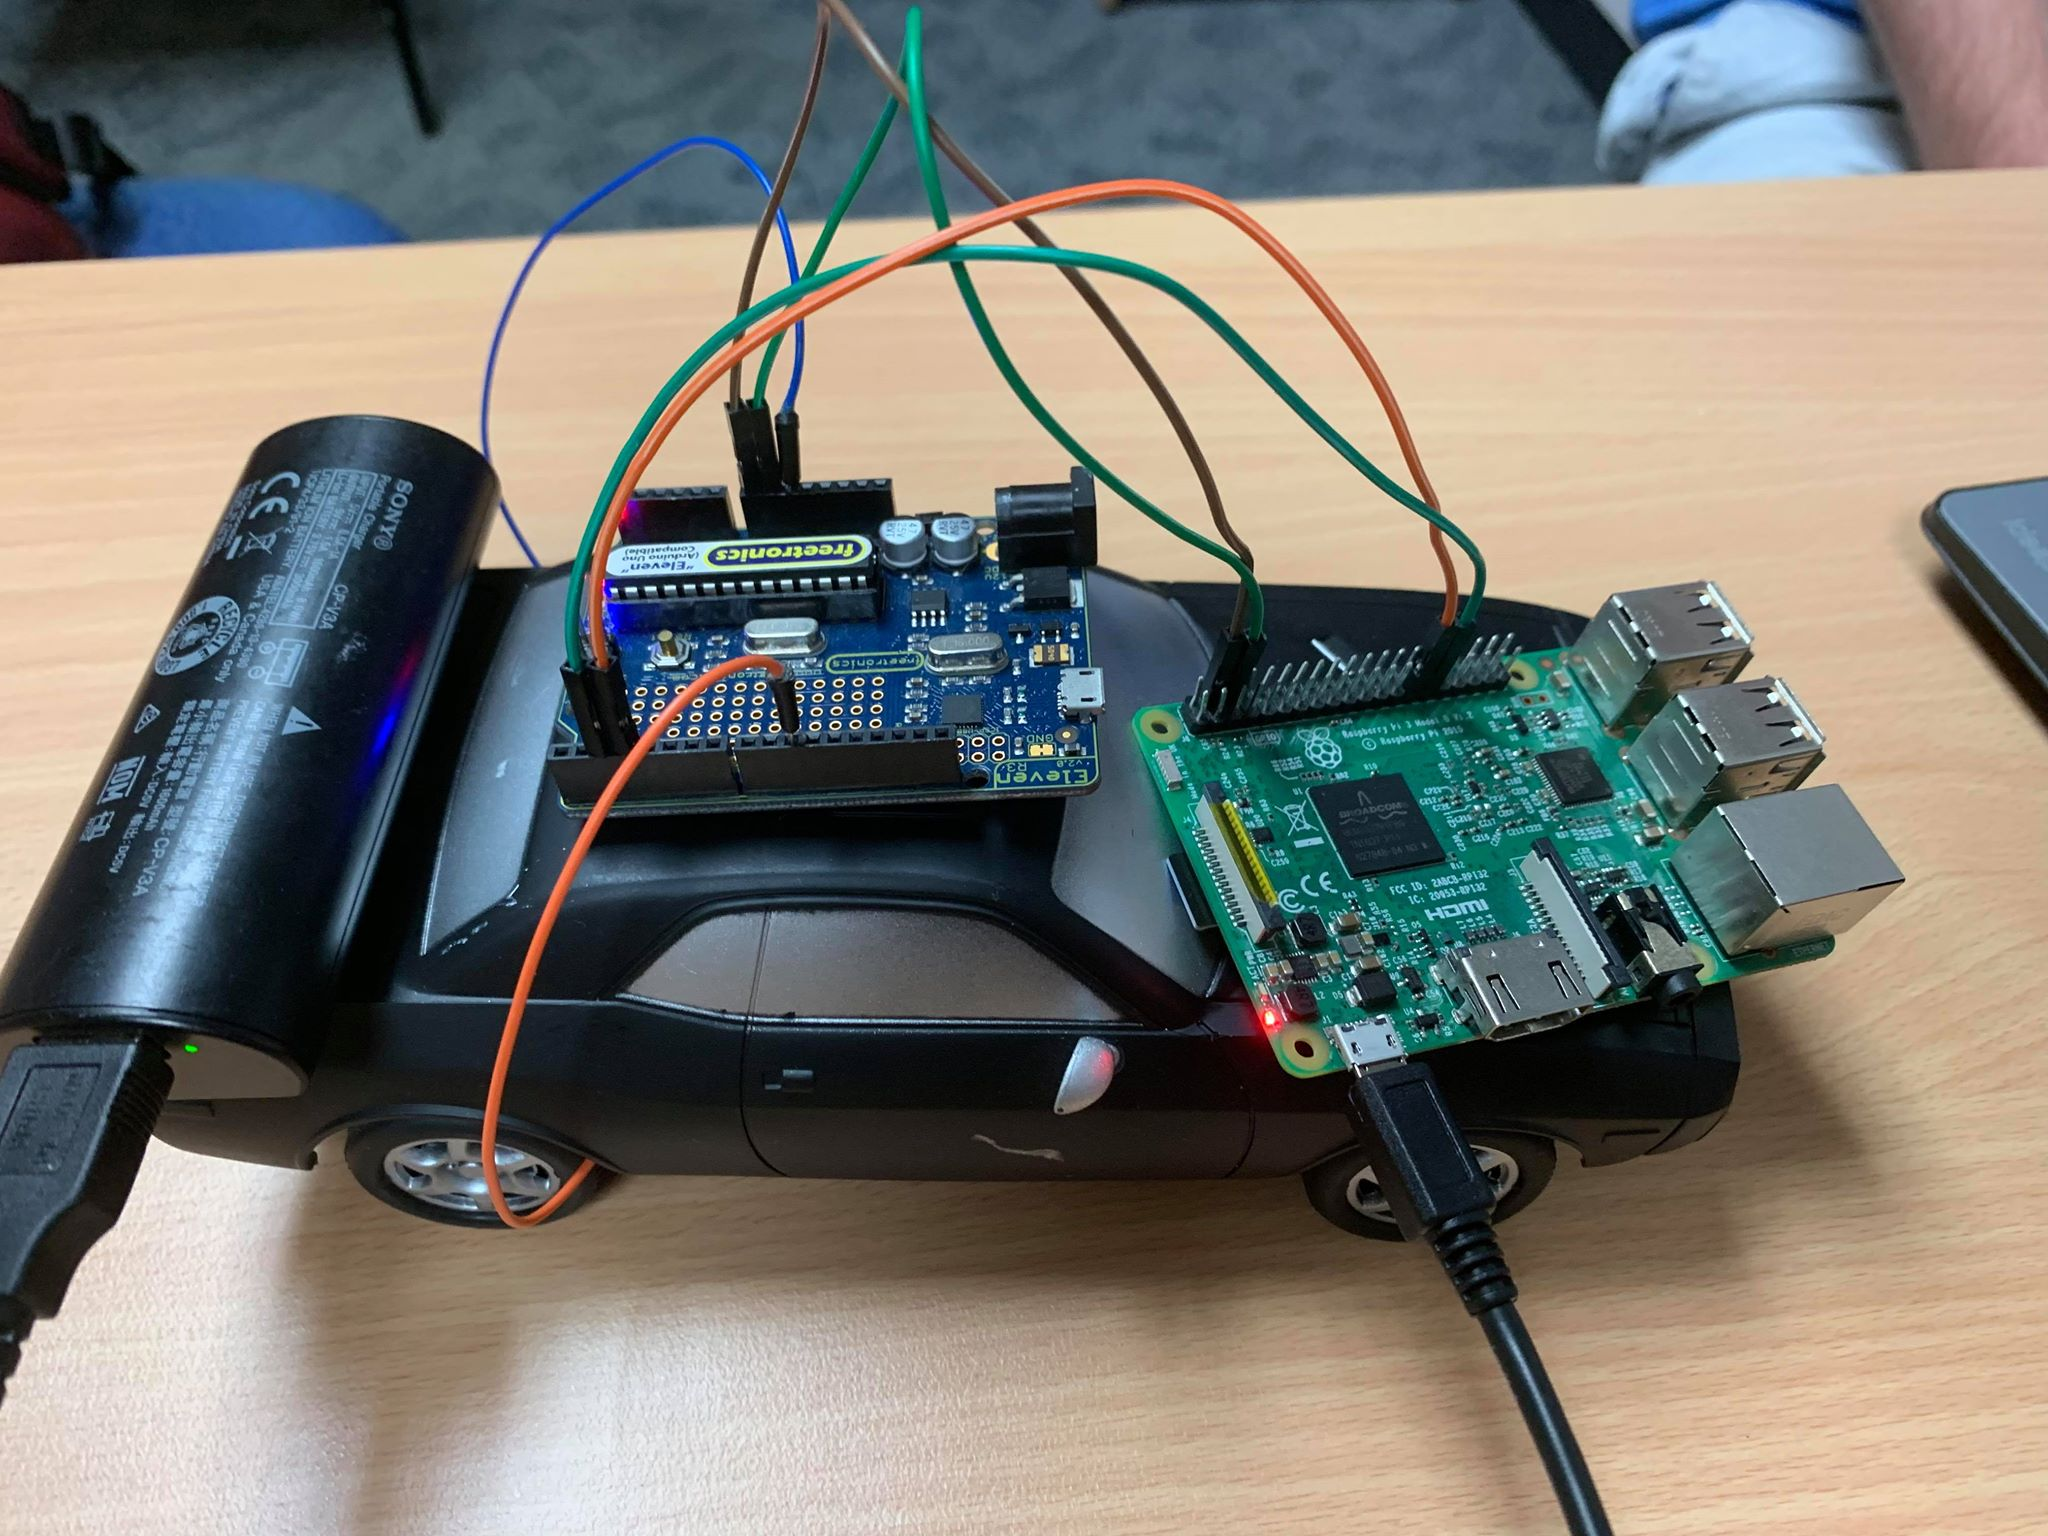
\includegraphics[height=7cm, width=7cm]{figures/CarWithRaspberryPi.jpg}
	\caption{Prototype vehicle with Raspberry Pi and Arduino UNO attached}
	\label{fig:CarWithRaspberryPi} 	
\end{figure}

\newpage

%      %%%%%
%    %%%%%%%%%
%   %%%     %%%
%   %%%     %%%
%   %%%     %%%
%      %%%%%
%   %%%%%%%%%%
%   %%%     %%%
%   %%%     %%%
%   %%%     %%%
%    %%%%%%%%%
%      %%%%%
%
%
% -----------------------------------------------------------------------------------------------
%

\subsection{Software}
Given that we have essentially no limitations on what we can use on the software side given the versatility of the Raspberry Pi, we have opted to use the Python programming language given it’s ease of use when it comes to developing and deploying. As well as this, it by far has the most libraries for Artificial Intelligence, Tensorflow being the most well known, and the one we will be using. This allows us to focus on applying the algorithms seamlessly instead of spending too much time on implementations that will surely be less performant than the heavily optimised existing frameworks.
\\\\
Creating an effective simulation will require emulating various real world situations in order to be effective. Using a game engine is ideal for this situation as they come with components for rendering and physics out of the box. Unity is the most well documented engine we found and is touted to be easy to learn compared to alternatives. Such alternatives include Godot, Unreal and CryEngine, however these all have less online documentation and are generally more complex than what we will need in this project. Unity also has components that help with linking up our Python based AI, making it much easier. Unity is the best option for our needs, so we will be learning it, and implementing our simulation with it.

\section{Activity Plan / Timetable}
Following the advice of the lecturer, our group will place emphasis on creating a software solution in conjunction with the creation a hardware solution. Each team member will have their own tasks and deadlines; some tasks will require collaborative work to meet deadlines. All team members have strong programming skills, though one member has more knowledge in robotics than the others. Each member will be involved in the production of hardware / software solution.
\\\\
Gantt Charts have been created for both semesters outlining the tasks that need to be completed and expected deadlines. Each task has been allocated time generously, though there is an option to push back work to the second semester as a last resort.

%      %%%%%
%    %%%%%%%%%
%   %%%     %%%
%   %%%     %%%
%   %%%     %%%
%   %%%     %%%
%    %%%%%%%%%%
%      %%%%% %%
%           %%%
%   %%%     %%%
%    %%%%%%%%%
%      %%%%%
%
%
% -----------------------------------------------------------------------------------------------
%



\begin{figure}
	\centering
	
	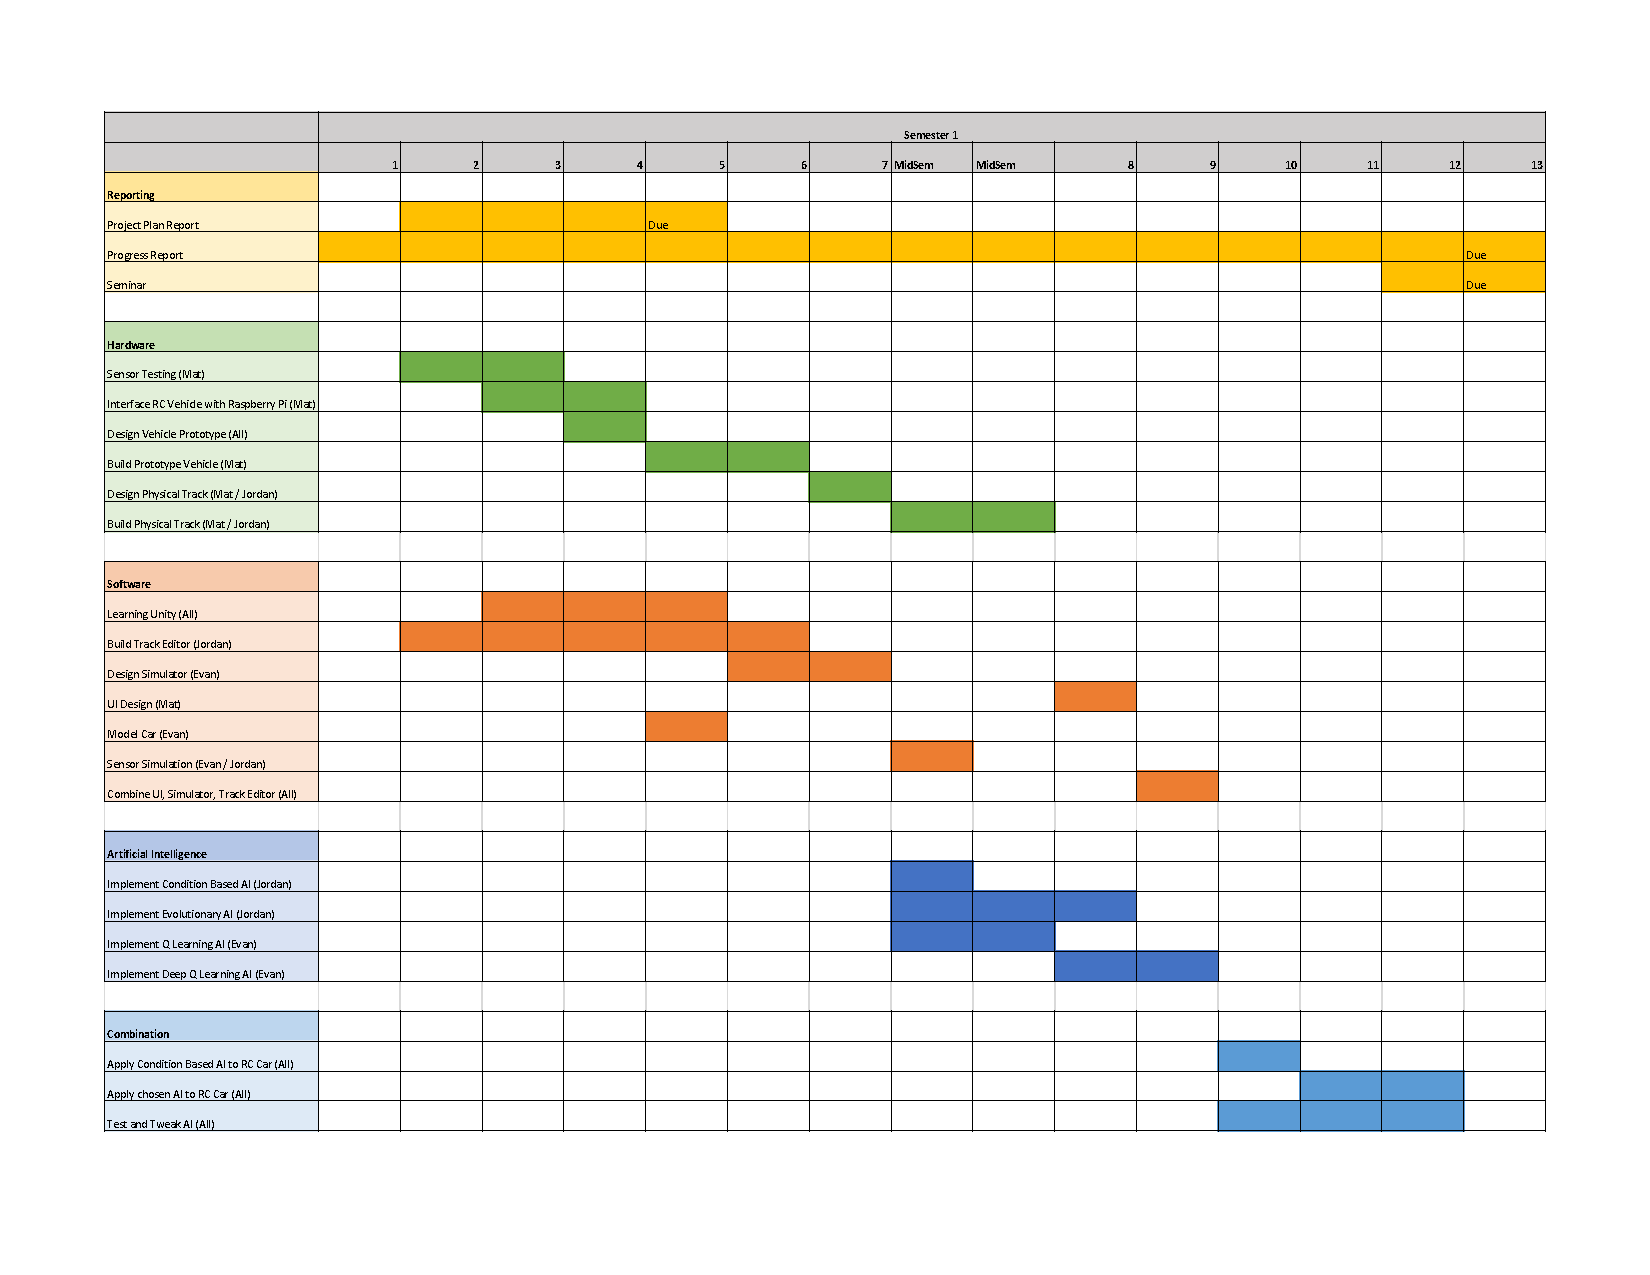
\includegraphics[width=23cm, height = 20cm, angle=90]{figures/TimelineSem1_2.pdf}
	\caption{Expected Timeline for Semester 1}
\end{figure}




%      %%%  	    %%%%%
%     %%%%		  %%%%%%%%%
%    %%%%%		 %%%     %%%
%   %%%%%%		 %%%     %%%
%      %%%		 %%%     %%%
%      %%%		 %%%     %%%
%      %%%		 %%%     %%%
%      %%%		 %%%     %%%
%      %%%		 %%%     %%%
%      %%%		 %%%     %%%
%   %%%%%%%%%	  %%%%%%%%%
%   %%%%%%%%%	    %%%%%
%
%
% -----------------------------------------------------------------------------------------------
%
\begin{figure}
	\centering
	
	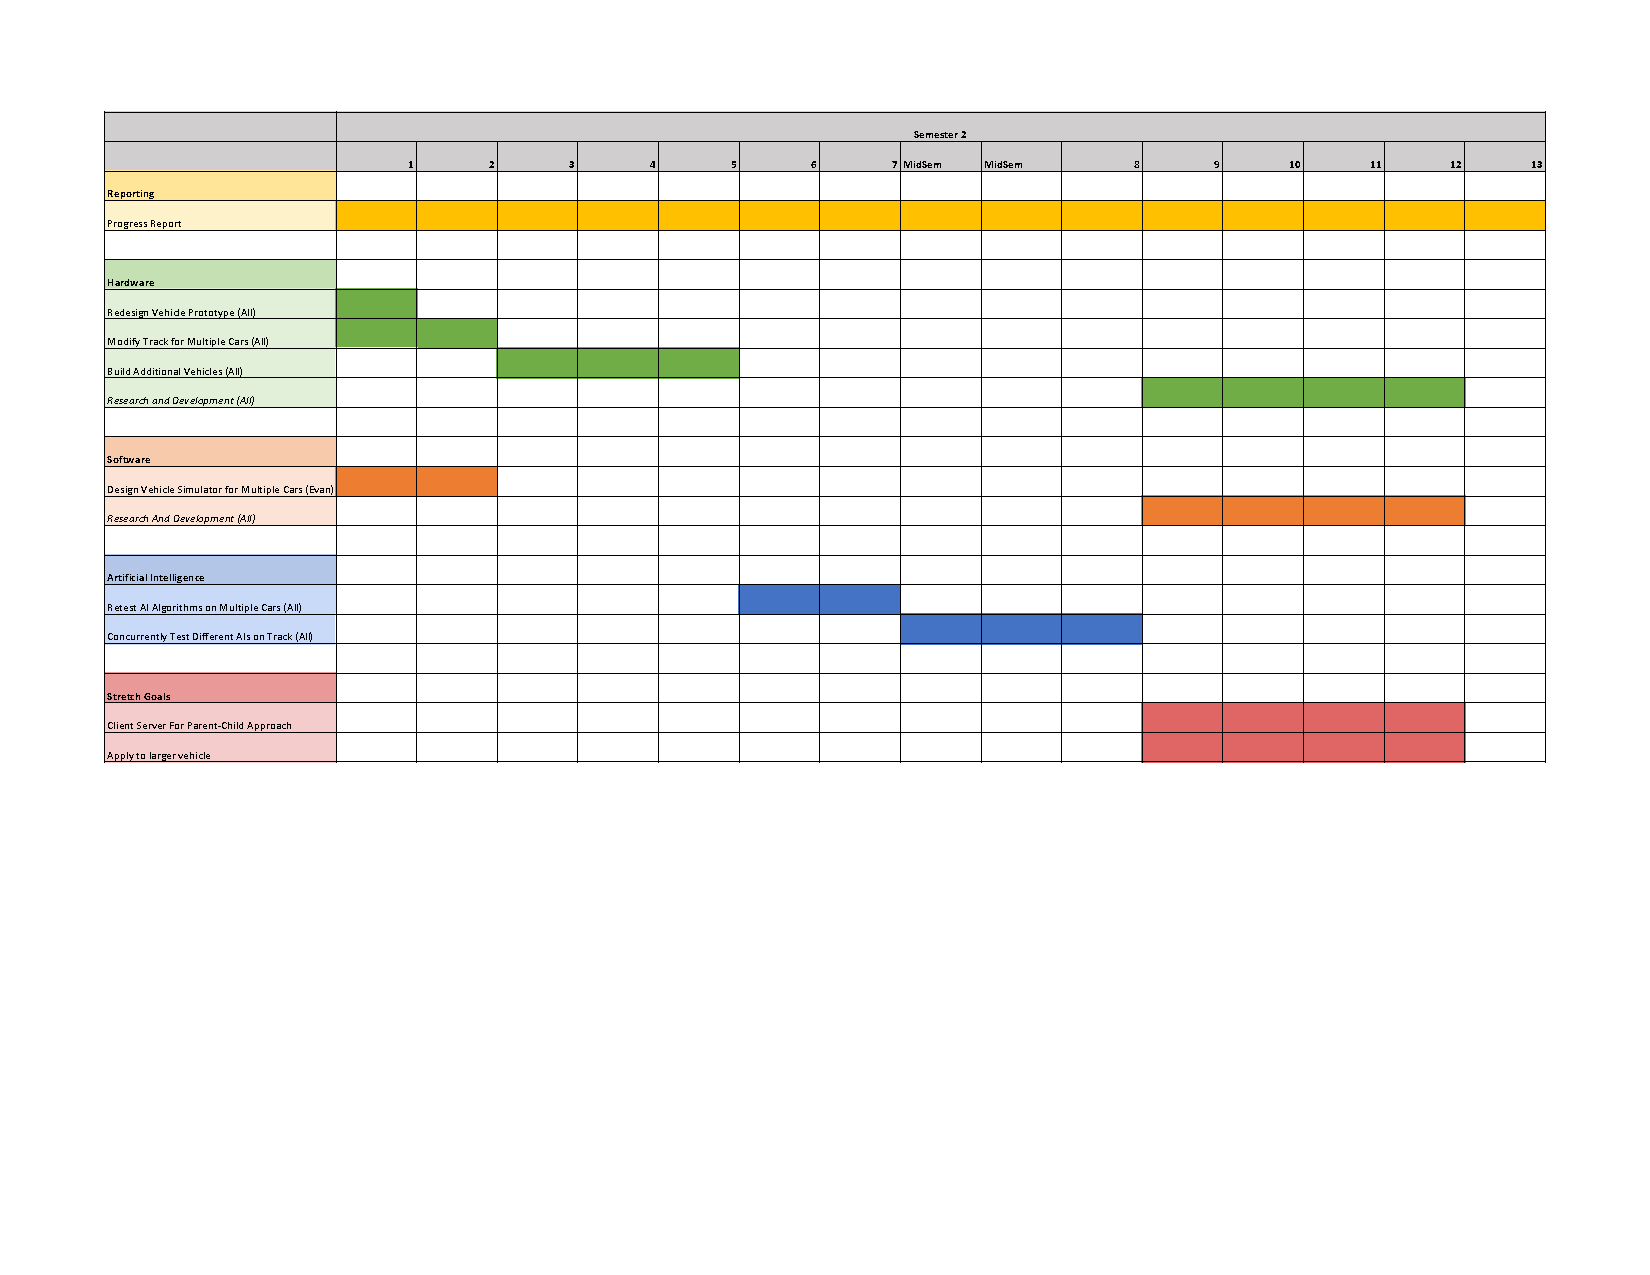
\includegraphics[width=23cm, height = 20cm, angle=90]{figures/TimelineSem2_2.pdf}
	\caption{Expected Timeline for Semester 2}
\end{figure}


\newpage



%      %%%  	    %%%  
%     %%%%		   %%%%	
%    %%%%%		  %%%%%	
%   %%%%%%		 %%%%%%	
%      %%%		    %%%	
%      %%%		    %%%	
%      %%%		    %%%	
%      %%%		    %%%	
%      %%%		    %%%	
%      %%%		    %%%	
%   %%%%%%%%%	 %%%%%%%%%
%   %%%%%%%%%	 %%%%%%%%%
%
%
% -----------------------------------------------------------------------------------------------
%

\subsection{Semester 1 Milestones}

\subsubsection{Reporting}
\textbf{Project Plan Report (All Members)}  – This milestone is part of the assessed items in this course that must be delivered by week 5. This has been allocated time starting from week 3 through to the due date. The group is continuously adapting our major project (initially considering to build our own vehicle rather than buying an off-the-shelf vehicle).
\\\\
\textbf{Progress Report (All Members)} – This will be kept by individual members in the form of a monthly journal. This journal is intended to outline their experiences, accomplishments and failures throughout the duration of the project.
\\\\
\textbf{Seminar (All Members)}– This is another milestone that is part of the assessed items of the course. At the end of the first semester, the group is expected to deliver a short presentation on our Work-Integrated Learning topic. Once our first prototype is to a state that can be demonstrated, the group will spend the final weeks of the semester preparing for the presentation. Two weeks will be sufficient time to prepare a speech and create demonstration videos for the project.


\subsubsection{Hardware}
\textbf{Sensor Testing (Mathew)} - Mathew will be conducting individual sensor testing before building the first prototype. This will give us background knowledge to determine what sensors are best suited for this task (Accelerometers, Infrared sensors, Ultrasonic Sensors, etc.). Two weeks should be sufficient time to research individual components and determine their benefits for this project.
\\\\
\textbf{Interface RC Vehicle with Raspberry Pi (Mathew)} - In order to control the vehicle, the Raspberry Pi will need to connect with it’s circuitry. This process will be time consuming, as the team will need to research this process, as well as allow additional time for debugging. Once successfully completed, this should deliver a fast response time and precise control over the vehicle’s motors.
\\\\
\textbf{Design Vehicle Prototype(Mathew/ Jordan)} - Once we have determined the appropriate sensors for the RC vehicle, the next step is to decide on the chassis. A vehicle could be designed and constructed by the team, or a cheaper and quicker alternative is to buy a RC car from a retail outlet. The vehicle must be large enough to support a Raspberry Pi, as well as additional components (Breadboard, sensors, wires, etc.) 3D printing is an avenue worthy of exploration for mounting purposes. This small milestone should take less than a week to complete.
\\\\
\textbf{Build Vehicle Prototype (Mathew/ Jordan)} - Following the design and construction, sensors and other required electronics will be mounted to the car (possibly including 3D-printed mounts). This milestone should be able to be completed shortly after designing the vehicle prototype.
\\\\
\textbf{Design Race Track (Mathew / Jordan)} - Our vehicle prototype will need a track in order to train and improve. The track will need to be constructed out of a material that is cheap, sturdy, modifiable. Constructing multiple tracks is essential in the training stage, such that the vehicle does not overfit to a specific track. Materials such as wood, brick, or cardboard are to be considered. Whilst designing physical tracks is a small task to complete, this milestone must give consideration to the chosen material - it must be easily obtainable, sturdy and within an acceptable budget.
\\\\

\newpage


%      %%%  	    %%%%%
%     %%%%		  %%%%%%%%%
%    %%%%%		 %%%     %%%
%   %%%%%%		         %%%
%      %%%		         %%%
%      %%%		    %%%%%%%
%      %%%		  %%%%%%%
%      %%%		 %%%
%      %%%		 %%%
%      %%%		 %%%
%   %%%%%%%%%	 %%%%%%%%%%%
%   %%%%%%%%%	 %%%%%%%%%%%
%
%
% -----------------------------------------------------------------------------------------------
%

\textbf{Build Race Track (Mathew  / Jordan)} - The race track will be assembled at one of the team member’s house. It is planned to test the track with an unmodified RC car to determine the track robustness and difficulty.

\subsubsection{Software}
\textbf{Learning Unity (All)} - For this project, the team will be using Unity to create most of the software tools required (Race Track Editor, Car Simulation, Artificial Intelligence implementations). A 2D engine was originally considered, though it would not be able to accurately simulate the required physics of  a digital vehicle. Unity was selected over other 3D engines due to its’ intuitive design. There are a variety of tutorials provided by the company to help new users. Two weeks has been allocated to learning the basics of the Unity Engine, which includes modelling, creating scripts, etc. C\# is used for creating the backend scripts, which is syntactically similar to Java, a language that all team members are familiar with throughout their time at university.
\\\\
\textbf{Design Car Simulator (Evan)} - To test multiple artificial intelligence algorithms, a program must be designed to closely simulate the motion and control of the RC car. A 3D development engine will be more beneficial as compared to a 2D engine, as this will allow the RC car to be modelled in 3D space. This will be in line with the desired end result. Two weeks has been allocated for this milestone to allow sufficient time to model the vehicle being used, as well as refine technical details about the car’s movement.
\\\\
\textbf{Building the Track Editor (Jordan)} - The car will learn to drive around tracks built by the user. Tracks need to be generated easily by the user such that the car can train and improve over multiple tracks, preventing overfitting behaviour. Ideally, the user would be able to freehand draw a circuit with their mouse, and a track can be automatically generated with a predetermined width. Alternatively, the user can draw the edges of the track using a Polygon tool. The track editor has been allocated three weeks for completion. This has taken extra time into account in the event of unexpected issues or other time commitments.
\\\\
\textbf{UI Design (Mathew)} - The User Interface will be the final aspect of the software solution, creating a main menu screen for users, as well as additional functionality. The design of this interface will need to be minimal and clear for users. This milestone has been generously allocated two weeks for its completion; a draft interface is anticipated to be completed in the first week of this milestone and improvements can be added at a later date.
\\\\
\textbf{Sensor Simulation (Evan / Jordan)} - The software tool should not only closely represent how the car moves and interacts with the environment; it must also simulate the electronic sensors that will be used in the physical prototype. In order for the Artificial Intelligence algorithms to train and improve, it must be able to receive data from the sensors.
\\\\
One of the main purposes of this milestone is to determine whether the Artificial Intelligence will be able to learn with incomplete information gathered from the environment. The AI will not have access to the vehicle’s current speed, current position on the track and drift velocity (if possible), as well as having a limited field of view of obstacles placed on the track.
\\\\
There is the ability to buy additional sensors that will rectify this issue, though budget constraints and physical placement must be taken into consideration for this project.

\newpage

%      %%%  	    %%%%%
%     %%%%		  %%%%%%%%%
%    %%%%%		 %%%     %%%
%   %%%%%%		         %%%
%      %%%		         %%%
%      %%%		    %%%%%%%
%      %%%		    %%%%%%%
%      %%%		         %%%
%      %%%		         %%%
%      %%%		 %%%     %%%
%   %%%%%%%%%	  %%%%%%%%%
%   %%%%%%%%%	    %%%%%    
%
%
% -----------------------------------------------------------------------------------------------
%


\textbf{Combine UI, Simulator, Track Editor (All)} - This process will involve combining individual elements of the software solution into one main package. Various 3D development engines use ‘scenes’ as a basis for creating a level, where one scene can link to another after its completion. This will be a similar process for our software solution, where a main menu will link to the track editor section, or the simulation section. One week has been allocated (as a maximum), though this milestone should be completed very quickly if everything performs as expected.



\subsubsection{Artificial Intelligence}
\textbf{Implement Conditional Based AI (Jordan)} - This AI will be a looping structure that will include conditions and statements to determine what action the vehicle will perform. For example, if the distance to a wall on the left side of the vehicle is less than 5cm, then the vehicle should turn to the right. This will be the benchmark algorithm. One week will be enough time to complete this conditional AI, which will include applying the AI script to the simulated car.
\\\\
\textbf{Implement Evolutionary AI (Jordan)} - A combination of genetic algorithms and neural networks will be used to determine if an optimal solution can appear through evolution. The software simulation will be able to emulate many cars at once, which is ideal as replicating the algorithm on the physical RC car cannot be completed in a timely manner. If the simulation is closely comparable to the physical vehicle, it would be possible to transfer the AI to the RC car, however it is more interesting if the learning took place on the car. Three weeks will also be allocated for this milestone, previous knowledge from other university courses will provide insight to complete this AI.
\\\\
\textbf{Implement Q Learning Algorithm (Evan)} - Q Learning\cite{QLearningRobotControl} is a reinforcement learning algorithm, indicating what action must be completed in a specific circumstance. This algorithm will be implemented using Q Tables\cite{QLearningTabular}. A tabular solution needs to have a finite input space, which can be calculated by (number of possible inputs from the distance sensor) \^ (number of distance sensors used). The distance sensors will produce an infinite range of possible distance values, though it can be reduced by determining equivalence classes. This milestone will have two weeks to be completed, previous knowledge will also help in completing this AI. 
\\\\
\textbf{Implement Deep Q Learning Algorithm (Evan)} -  Deep Q Learning\cite{DeepQLearning} is the application of Neural Networks to Q Learning. Neural networks will be able to handle the infinite input space problem in regular Q Learning. There are many further advanced Q Learning Structures such as Double Deep Q Learning, Duelling Deep Q Learning, but for this project we will focus on Deep Q Learning. This will require using the TensorFlow library, which isn’t ideal as the Raspberry Pi has limited processing power.

\subsubsection{Combination}

\textbf{Apply Conditional Based AI to RC Car (All)} - Once the software solution is completed and tested, the team will be applying the Conditional Based AI to the physical car. This milestone should be completed within a week, though it may be implemented earlier in the semester depending on the difficulty of other milestones.
\\\\
\textbf{Apply Chosen AI to RC Car (All)} - After running all AIs in the simulation, the team will determine the best AI to apply to the RC car. It is not known which AI will emerge victorious. Two weeks will be used to test other AIs on the RC car, as well as allowing enough time for the Evolutionary Algorithm to be fairly tested. 

\newpage


%      %%%  	        %%%
%     %%%%		       %%%
%    %%%%%		      %%%
%   %%%%%%		     %%%
%      %%%		    %%%
%      %%%		   %%% %%%
%      %%%		  %%%  %%%
%      %%%		 %%%%%%%%%%%
%      %%%		 %%%%%%%%%%%
%      %%%		       %%%   
%   %%%%%%%%%	       %%%   
%   %%%%%%%%%	       %%%    
%
%
% -----------------------------------------------------------------------------------------------
%

\textbf{Test and Tweak AI (All)} - If the AI is not performing as expected once applied to the RC Car, the team can explore the possibility of tweaking the AI to improve performance. The lead-up weeks to the end of the first semester will be used for this milestone, as well as working on final reports and the presentation.

\subsection{Semester 2 Milestones}


\subsubsection{Reporting}
\textbf{Progress Report (All)} - Following from Semester 1, each team member will keep a journal to show their progress through the second half of this project. Any ideas, notes, successes and failures will be documented.

\subsubsection{Hardware}
\textbf{Redesign Vehicle Prototype (All)} - With the knowledge acquired from the first semester, the team will investigate improving the first prototype. This may involve purchasing a new vehicle chassis, using different mounting strategies, etc. It is unknown at the stage of writing this report if the first prototype will need any improvements, though one week has been allocated to explore different prototype strategies.
\\\\
\textbf{Modify Track for Multiple Cars (All)} - In the second semester, the team would like to trial multiple cars driving on a track simultaneously. The predesigned track will need to be widened to allow for more vehicles on the track at once. Two weeks will be allocated as a maximum to redesign a track.
\\\\
\textbf{Build Additional Vehicles (All)} - Each team member owns as Raspberry Pi that will be used as the \emph{brain} for more RC cars. To remain consistent, the same RC car models will need to be purchased. Sensors, wires and other electronics will need to be sourced from local vendors. The process of building more cars will take significantly less time, as the building process will be documented from the first semester. This milestone will take two weeks to complete. On completion, the team will have three more vehicles that can be used in training. 
\\\\
\textbf{Research and Development (All)} - This may involve researching different sensors, utilising cameras or looking into different vehicle models. This milestone will use the remaining four weeks of the semester, though if another milestone becomes high priority, Research and Development can be paused. 

\subsubsection{Software}
\textbf{Design Vehicle Simulator for Multiple Cars (Evan)} - This milestone will expand on the existing software solution to allow multiple simulated cars to train at the same time. Each car will have its own AI, such that users can see real time differences as the AIs are learning. This milestone will be quick to complete in two weeks; some scripts will need to be tweaked and the simulator will need to use a wider track.
\\\\
\textbf{Research and Development (All)} - This may involve expanding the existing software solution, possibly implementing new Artificial Intelligence algorithms. This milestone will use the remaining four weeks of the semester, though if another milestone becomes high priority, Research and Development can be paused. 

\newpage

%      %%%   	%%%%%%%%%%%
%     %%%%	 	%%%%%%%%%%%
%    %%%%%	 	%%% 
%   %%%%%%	 	%%%
%      %%%	 	%% %%%%%
%      %%%	 	%%%%%%%%%%
%      %%%	 	        %%%
%      %%%	 	        %%%
%      %%%	 	        %%%
%      %%%	 	%%%     %%%
%   %%%%%%%%% 	 %%%%%%%%%
%   %%%%%%%%% 	   %%%%%
%
%
% -----------------------------------------------------------------------------------------------
%
\subsubsection{Artificial Intelligence}
\textbf{Retest AI Algorithms on Multiple Cars (All)} - Once the new vehicles are built, we can begin to apply different AI algorithms to different cars and see how the algorithm handles driving with other vehicles. Two weeks will be allocated to test each algorithm and determine results.
\\\\
\textbf{Concurrently Test Different AIs on Track (All)} - This milestone expands from the preceding milestone, where different AI algorithms will be applied to different cars. Users will be able to compare and observe as the different AIs attempt to navigate a track. Two weeks has been allocated for this milestone as sufficient time to determine a victorious algorithm.

\subsubsection{Stretch Goals}
\textbf{Application of Client-Server Model to Raspberry Pis} - Rather than having multiple Raspberry Pi’s independently learning, we could localise all training on a central computer and send out signals to the Raspberry Pis from the computer. This way, training could be achieved at a much higher rate at the cost of latency. This is still a possibility to look into at a later date.
\\\\
\textbf{Apply to larger vehicle} - Since this project has been working with small RC cars, it would be interesting to see how the AI would work on a larger RC vehicle. These larger vehicles would cost more, though could potentially show more rewarding results. 


\subsection{Project Feasibility}
In terms of feasibility, this project will include challenges for all team members. Though there are many complex tasks involved in this project, it is believed that the semester 1 timeline  is realistic and achievable. There is also an option to push certain milestones into the second semester (though this is not ideal).


\newpage




%      %%%   	   %%%%%
%     %%%%	 	 %%%%%%%%%
%    %%%%%	 	%%%     %%%
%   %%%%%%	 	%%%
%      %%%	 	%% %%%%%
%      %%%	 	%%%%%%%%%%
%      %%%	 	%%%     %%%
%      %%%	 	%%%     %%%
%      %%%	 	%%%     %%%
%      %%%	 	%%%     %%%
%   %%%%%%%%% 	 %%%%%%%%%
%   %%%%%%%%% 	   %%%%%
%
%
% -----------------------------------------------------------------------------------------------
%

\section{Ethics Considerations}
For this project, there are little to no ethics clearances required, though there are still some ethical considerations to examine.

\subsection{Self Driving Vehicles}
Self driving vehicles is a hot topic for ethical debate - who is to blame if there is an accident in a self-driving car? This project is scaled down immensely from the self-driving car debate.  Our project focuses on applying artificial intelligence to a small RC Car. 
\\\\
Due to the size of the RC Car, it will not cause any hazards or damage to humans or property in the event of an ‘accident’. The vehicle will hold a Raspberry Pi, sensors and various cables that will be secured properly. 
\\\\
By creating a physical track out of materials to form barriers, the car will not be able to leave the track by itself during operation. 

\subsection{Data and Consent}
Data is planned to be gathered from ultrasonic sensors, meaning that there will be no need for human interaction or human consent of data. If the project expands to include cameras as sensors, we will need to create informed consent forms to allow the recording of humans whilst the RC car is driving. Human faces can be blurred if required.

\subsection{Data Bias}
Avoiding Data Bias is a primary goal throughout this project. As the group is planning to work with and compare multiple machine learning algorithms, it will be crucial to minimise any sort of human bias that could possibly be introduced into the project. We will need to properly define the criteria for comparing the different AI algorithms, such that it does not encourage favouritism to a particular algorithm.

\newpage


%      %%%   	%%%%%%%%%%%
%     %%%%	 	%%%%%%%%%%%
%    %%%%%	 	        %%%
%   %%%%%%	 	        %%%
%      %%%	 	       %%%
%      %%%	 	      %%%
%      %%%	 	     %%%
%      %%%	 	    %%%
%      %%%	 	    %%%
%      %%%	 	    %%% 
%   %%%%%%%%% 	    %%%
%   %%%%%%%%% 	    %%%
%
%
% -----------------------------------------------------------------------------------------------
% 

\section{Statement of individual contribution}
Each member was allocated a section to write about in this report. All team members were involved in the process of creating a title and writing a summary about the project. Each member was available to lend a hand in other member’s sections if they were lost for words.
\\\\
\emph{Mathew} wrote the Background section outlining the reason why the team decided to complete a project on this topic. Mathew also wrote about the approach the team will take to complete the project. The process of testing multiple artificial intelligence techniques will determine if there is a victorious algorithm, which can be applied to the RC Vehicle.
\\\\
\emph{Evan} wrote about the Aims and Expected outcomes in the project. This provided a stage-by-stage plan on what our goals are with this project and provided an insight on how we will be able to complete them. Evan is taking a managerial position in this project, as he is the most experienced with artificial intelligence and to gain project management skills.
\\\\
\emph{Jordan} wrote the Activity Plan / Timetable section. Each group member was involved in designing the Gantt Charts for Semester 1 and Semester 2, allocating each member assigned tasks that are expected to be completed in various weeks. Jordan expanded on each milestone found in the Gantt Charts, explaining what must be achieved to complete the milestone. This includes any ethical considerations that might emerge during the project. Jordan formatted the document in Latex.


\newpage



%      %%%   	    %%%%%
%     %%%%	 	  %%%%%%%%%
%    %%%%%	 	 %%%     %%%
%   %%%%%%	 	 %%%     %%%
%      %%%	 	 %%%     %%%
%      %%%	 	    %%%%%
%      %%%	 	 %%%%%%%%%%
%      %%%	 	 %%%     %%%
%      %%%	 	 %%%     %%%
%      %%%	 	 %%%     %%%
%   %%%%%%%%% 	  %%%%%%%%%
%   %%%%%%%%% 	    %%%%%
%
%
% -----------------------------------------------------------------------------------------------
%



%code example
%\vspace{10pt}
%\begin{lstlisting}
%    #include <iostream>
%    using namespace std;
%
%    int main() {
%    	cout << "Hello World" << endl;
%    	return 0;
%    }
%\end{lstlisting}
%\vspace{5pt}




%
% ---- BIBTEX STUFF -----------------------------------------------------------------------------
%\bibliographystyle{plain}

\bibliography{COMP3851AProjectPlanReport}
\bibliographystyle{ieeetr}

% -----------------------------------------------------------------------------------------------
%

\end{document}